{\large(a)}

\textbf{Gaussian filter and Gaussian blur}

I used the Gaussian filter to smoothen the image to reduce impact of noise in edge detection algorithms being used here. The Gaussian filter is used to blur the image. The filter is given by:

$$n_\sigma = \frac{1}{16} \times
\begin{bmatrix}
    1 & 2 & 1 \\
    2 & 4 & 2 \\
    1 & 2 & 1
\end{bmatrix}$$

This is reffered as Gaussian blur and is very often used in image processing.

\begin{figure}[H]
    \centering
    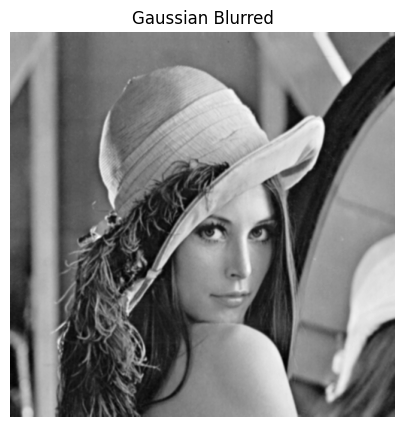
\includegraphics[width=.5\textwidth]{res/3a_gaussian.png}
    \caption{Gaussian filter applied to the original image}\label{fig:3a_gaussian}
    \label{fig:3d_gaussian}
\end{figure}

The result is slightly blurred as the kernel size is very small ($3\times3$). Image will get more blurry when we increase the kernel size, as the kernel would have more pixels to interact with.

{\large(b)}

\textbf{Laplacian filter}

The Laplacian filter is a second-order derivative filter used in image processing for edge detection and enhancement. It highlights regions of rapid intensity change, which correspond to edges in an image. I used the following laplacian filter that was taught in class:

$$\Delta^2 =
\begin{bmatrix}
    0 & 1 & 0 \\
    1 & -4 & 1 \\
    0 & 1 & 0
\end{bmatrix}$$

This filter is convolved with the image to produce the following image:

\begin{figure}[H]
    \centering
    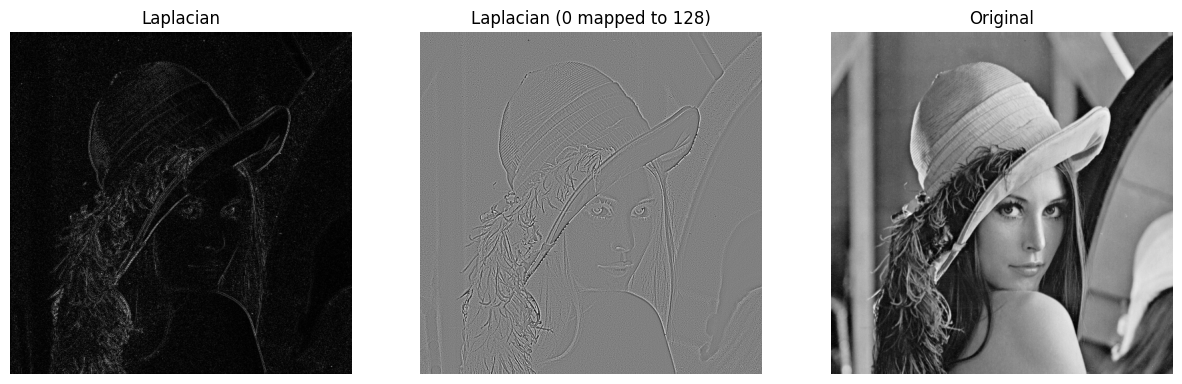
\includegraphics[width=1.06\textwidth]{res/3b_laplacian.png}
    \caption{Laplacian filter applied to the original image}
    \label{fig:3b_laplacian}
\end{figure}

\textbf{Zero crossing}

The way I implemented zero crossing here is for each pixel value $P_{i,j}$ I am checking if the sign is changed from previous pixels, that is $P_{i-1,j}$ and $P_{i,j-1}$. If the sign is changed then I am marking that pixel as edge pixel if the change between the pixels is greater than a certain threshold given to the function of zero crossing I have implemented.

As observed here, no matter how much I increase the zero crossing, the results are consistently noisy. This is because the image is noisy and the zero crossing is not able to detect the edges properly due to it's small size of kernel. Also, we would want to keep the threshold as low as possible, as more the threshold, more the edges will be lost.

\begin{figure}[H]
    \centering
    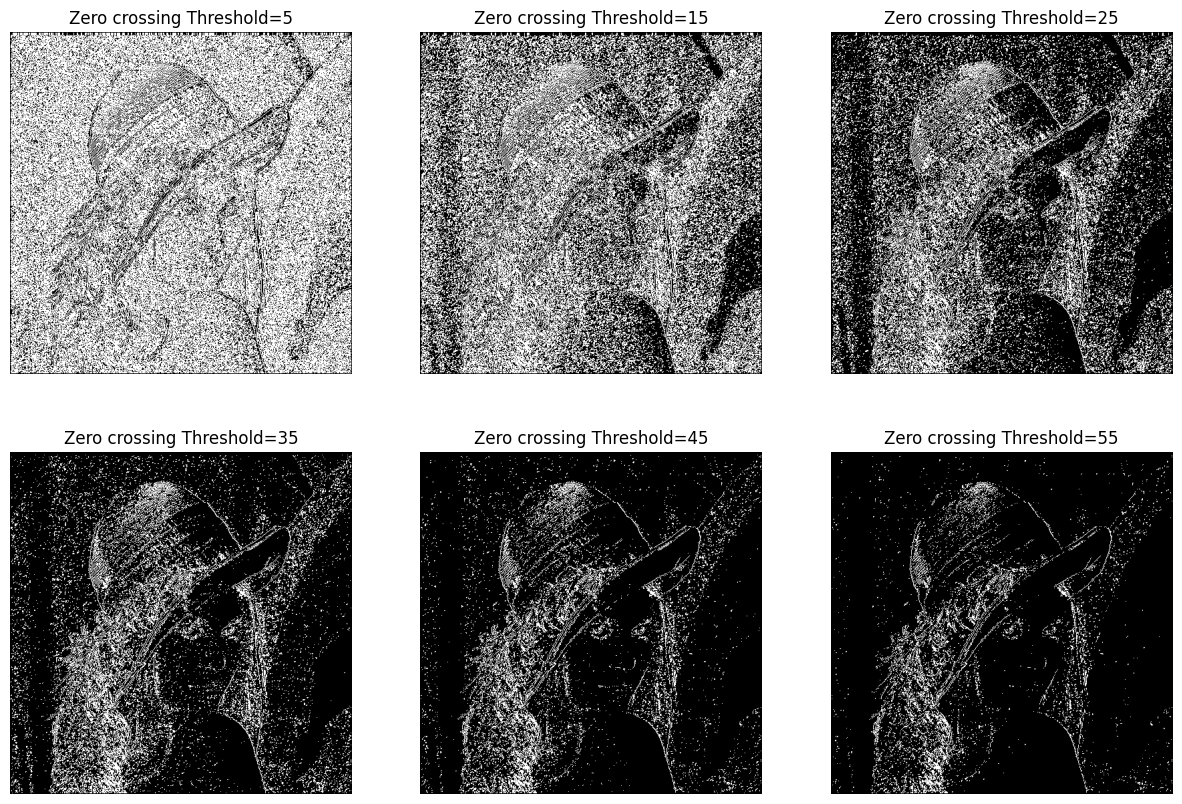
\includegraphics[width=1.06\textwidth]{res/3b_zero_crossing.png}
    \caption{Zero crossing applied to the laplacian image with different threshold}
    \label{fig:3b_zero_crossing}
\end{figure}

\textbf{Laplacian of Gaussian (LoG)}

To over come the issue of noise in the laplacian filtered image, we would want our main image to be our of noise, i.e., we want the original image to be smooth. This can be done using gaussian filter. The LoG is the convolution of the laplacian filter and the gaussian filter. The LoG is given by:

$$LoG*I = \Delta^2 * n_\sigma * I$$

\begin{figure}[H]
    \centering
    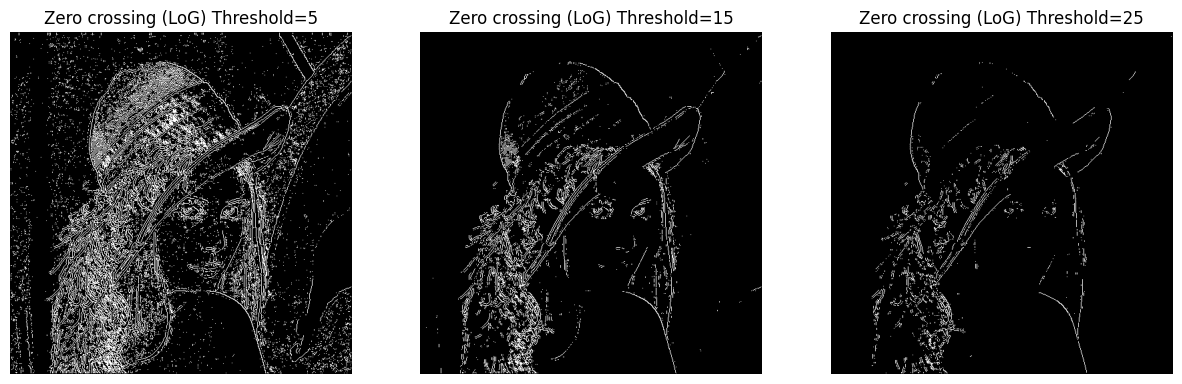
\includegraphics[width=1.06\textwidth]{res/3b_zero_crossing_log.png}
    \caption{LoG applied to the original image}
    \label{fig:3c_log}
\end{figure}

{\large(c)}

As you can see that we get very good results at $threshold=15$ only, compared to that of useless results with only laplacian filter. Here below is a side my side comparision of The original image, laplacian filter and LoG filter.

\begin{figure}
    \centering
    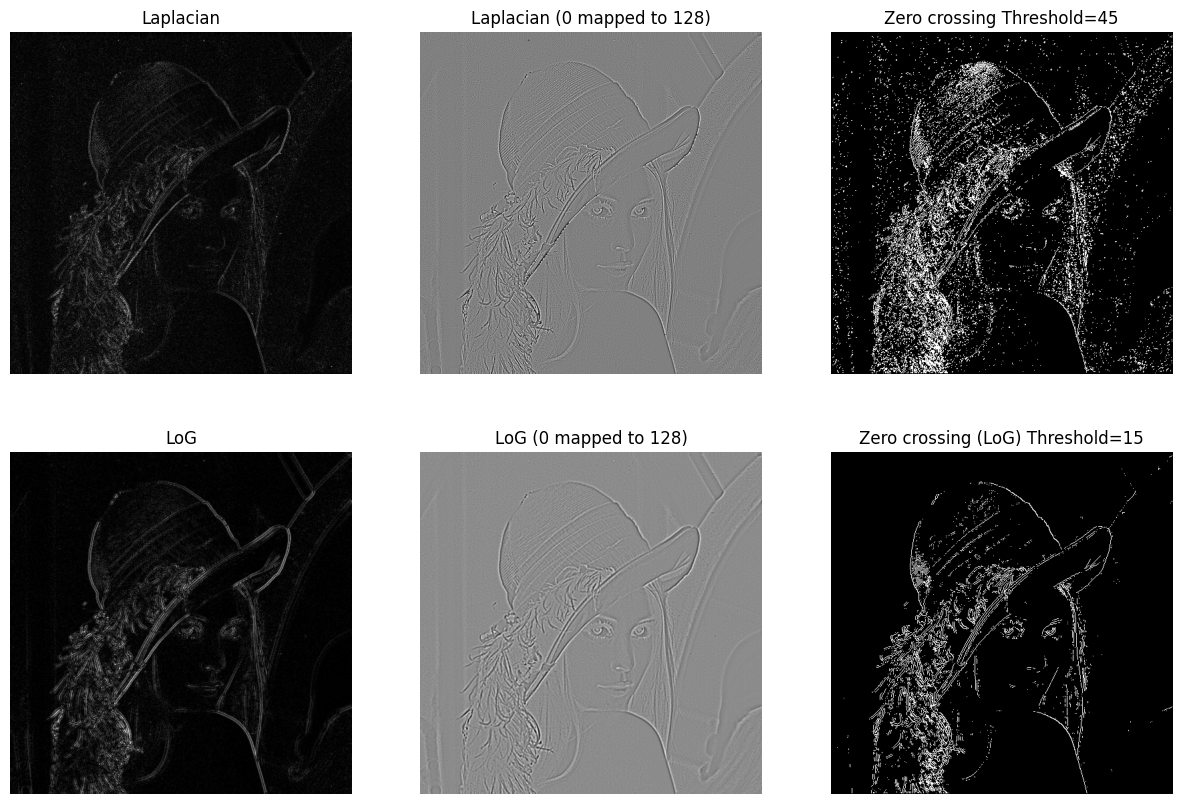
\includegraphics[width=1.06\textwidth]{res/3c_log_vs_lap.png}
    \caption{LoG vs Laplacian filter}
    \label{fig:3c_log_vs_lap}
\end{figure}